\section{Test-Circuit Results (Part C)}\label{sec:circuit}

\subsection{Method}\label{sec:circuit:method}
The adder is built only from the gates of Part~B (27 NAND2, 3 INV, 2 AND2, 1 OR2). For every one of the 64 input vectors the logic value at the inputs of every gate is computed by evaluating the gates in topological order; the computed sum bits and carry-out equal the correct 3-bit sum for all 64 vectors and agree with the SPICE output voltages (threshold $V_{DD}/2$) in all 12,800 simulations.
For each vector and corner $k$, every gate's ML leakage is looked up from the Part~B prediction table by (gate type, input bits, corner), and the circuit leakage is the plain sum
\begin{equation}
\hat I_{CLA}(v,k)=\sum_{g=1}^{33}\hat I_{g}\bigl(\text{type}_g,\ \text{inputs}_g(v),\ k\bigr),
\label{eq:cla}
\end{equation}
which assumes that every gate input sits at exactly 0 or $V_{DD}$ and ignores loading between gates, as the project document prescribes. The reference is the SPICE simulation of the complete transistor netlist (64 vectors $\times$ 200 corners $=$ 12,800 rows, corners identical to Part~B).
As a diagnostic we also compute the \emph{ceiling}: the same sum with the Part~B \emph{SPICE} gate leakages instead of the ML ones, i.e.\ with perfect gate models. It isolates what the summation itself costs.
% src: ml/evaluate_cla.py, results/partC/cla3_gates.csv, results/partC/cla3_predictions.csv

\subsection{Results}\label{sec:circuit:results}
The plain sum of the ML gate leakages predicts the circuit leakage with a mean accuracy of 99.00\,\% (median 99.17\,\%), a bias of $-0.23\,\%$, a 95th percentile of $|e|$ of 2.57\,\% and a maximum of 4.02\,\% over 12,800 simulations (Table~\ref{tab:cla}, Fig.~\ref{fig:claparity}). The per-vector accuracy lies between 98.95\,\% (vector $3+3$) and 99.05\,\% (vector $0+7$), the median $|e|$ between 0.77 and 0.89\,\%, and the median SPICE leakage per vector between $\SI{2.72e-6}{\ampere}$ and $\SI{3.56e-6}{\ampere}$; the per-vector table is provided in the project repository. The worst row is vector $1+7$ at corner 39 (\SI{122}{\celsius}), $+4.02\,\%$; no row exceeds 5\,\%, 5,172 of 12,800 exceed 1\,\%.
\textbf{The margin to the 99\,\% target is small.} The ceiling is 99.16\,\%: even with perfect gate models the sum of isolated gate leakages underestimates the circuit leakage by 0.66\,\% (median) and cannot exceed 99.16\,\% mean accuracy. The ML result of 99.00\,\% sits just below this ceiling because the ML gate errors have a small \emph{positive} bias that offsets the negative summation bias: the ML sum exceeds the ceiling sum by a median of $+0.70\,\%$ (mean $+0.81\,\%$), so the circuit bias is $-0.23\,\%$ against $-0.66\,\%$ for the ceiling; Part~C is not better than Part~B because the models are better there, but because the two errors partly cancel. The project document expects the circuit accuracy to be lower than the gate accuracy because of the neglected loading; here it is not (99.00\,\% against 98.87\,\%) for exactly this reason.
% src: results/partC/cla3_results.csv, results/partC/cla3_predictions.csv, results/analysis/report_numbers/error_breakdown_partC.csv, results/analysis/loading_analysis/cancellation_check.txt
\begin{table}[t]
\caption{3-bit CLA, final models: ML (sum of the ML gate leakages) and ceiling (sum of the SPICE gate leakages), 12,800 simulations.}
\label{tab:cla}
\centering\footnotesize
\setlength{\tabcolsep}{3pt}
\fitcol{% src: results/partC/cla3_results.csv (row ALL)
\begin{tabular}{lrr}
\toprule
Metric & ML (sum of ML gates) & Ceiling (sum of SPICE gates) \\
\midrule
SPICE median (A) & \num{2.99e-06} & \num{2.99e-06} \\
Estimate median (A) & \num{3.01e-06} & \num{2.97e-06} \\
Bias (\%) & -0.23 & -0.66 \\
Median $|e|$ (\%) & 0.83 & 0.66 \\
P95 $|e|$ (\%) & 2.57 & 2.11 \\
Max $|e|$ (\%) & 4.02 & 3.83 \\
\midrule
Mean accuracy (\%) & 99.00 & 99.16 \\
Median accuracy (\%) & 99.17 & 99.34 \\
\bottomrule
\end{tabular}
}
\end{table}
% Table IX (Sec. VII-C, VIII-A), placed here so that the two-column float reaches the page of its first reference
\begin{table*}[t]
\caption{Mean $|e|$ (\%) by corner condition: Part~B (ML) and Part~C (ML and ceiling), and the median signed error (bias) of Part~C. Temperature ranges in $^\circ$C, quartiles of the NMOS $V_{th0}$ and the PMOS $|V_{th0}|$, terciles of $V_{DD}$.}
\label{tab:breakdown}
\centering\footnotesize
% src: results/analysis/report_numbers/error_breakdown_partB.csv, error_breakdown_partC.csv
\begin{tabular}{llrrrrr}
\toprule
Variable & Range & B: mean $|e|$ & C: mean $|e|$ ML & C: ceiling & C: bias ML & C: bias ceil. \\
\midrule
temperature & -40--0.0 & 1.50 & 1.16 & 0.56 & +0.26 & -0.40 \\
 & 0.0--40.0 & 1.14 & 0.99 & 0.48 & +0.44 & -0.37 \\
 & 40.0--85.0 & 0.98 & 1.03 & 0.89 & -0.54 & -0.78 \\
 & 85.0--125.0 & 0.92 & 0.83 & 1.38 & -0.56 & -1.22 \\
\midrule
NMOS vth0 quartile & Q1 (lowest) & 1.34 & 1.19 & 1.20 & -0.90 & -1.04 \\
 & Q2 & 1.12 & 0.90 & 0.98 & -0.51 & -0.90 \\
 & Q3 & 0.98 & 0.91 & 0.72 & -0.11 & -0.54 \\
 & Q4 (highest) & 1.08 & 0.99 & 0.46 & +0.63 & -0.34 \\
\midrule
PMOS $|$vth0$|$ quartile & Q1 (lowest) & 1.25 & 1.22 & 0.74 & +0.05 & -0.58 \\
 & Q2 & 1.09 & 0.99 & 0.92 & -0.19 & -0.76 \\
 & Q3 & 1.16 & 0.94 & 0.89 & +0.04 & -0.72 \\
 & Q4 (highest) & 1.02 & 0.84 & 0.81 & -0.48 & -0.72 \\
\midrule
VDD tercile & low VDD & 0.84 & 0.82 & 0.70 & -0.46 & -0.55 \\
 & mid VDD & 1.00 & 0.98 & 0.80 & -0.20 & -0.65 \\
 & high VDD & 1.55 & 1.20 & 1.01 & +0.31 & -0.82 \\
\bottomrule
\end{tabular}

\end{table*}
\begin{figure}[t]
\centering
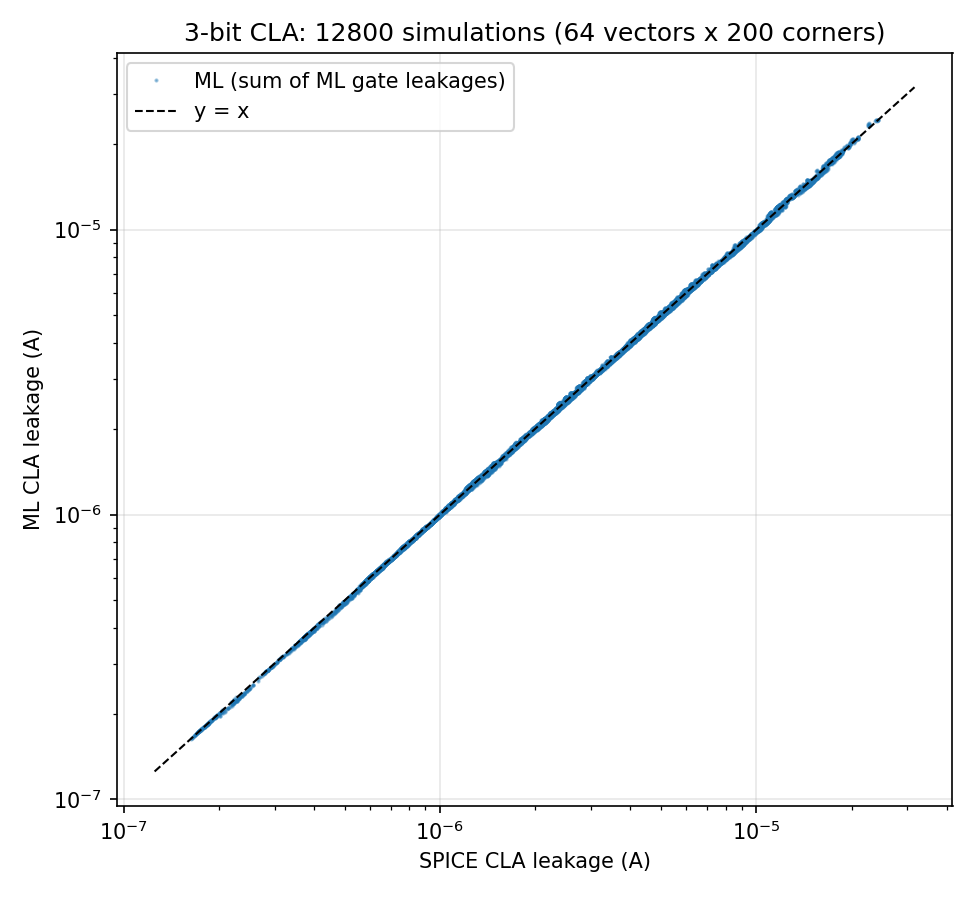
\includegraphics[width=\columnwidth]{figures/cla3_parity.png}
\caption{ML versus SPICE leakage of the 3-bit CLA for all 12,800 simulations (log axes, dashed line: ML $=$ SPICE).}
\label{fig:claparity}
% src: results/partC/cla3_parity.png
\end{figure}

\subsection{What limits the summation (ceiling analysis)}\label{sec:circuit:ceiling}
The ceiling error is not uniform: its mean $|e|$ grows from 0.56 and 0.48\,\% at $T\le40\,^\circ$C to 0.89 and 1.38\,\% at 40--85 and 85--125\,$^\circ$C, and its bias from $-0.40\,\%$ to $-1.22\,\%$ (Table~\ref{tab:breakdown}). The ML error does the opposite (1.16, 0.99, 1.03 and 0.83\,\%, bias $+0.26$, $+0.44$, $-0.54$, $-0.56\,\%$), which is again the cancellation described above.
Two contributions to the summation error can be identified. (i)~\emph{Loading:} in the isolated gate simulations the inputs are ideal sources, which supply (inputs at logic 1) or absorb (inputs at 0) a small gate current; in the circuit these currents flow through the driving gates. Adding the SPICE pin current of every input that is driven by another gate and is at logic 1 to the sum raises the ceiling from 99.16\,\% to 99.37\,\% (median 99.34 to 99.61\,\%, bias $-0.66$ to $-0.39\,\%$), i.e.\ it explains 0.21 of the 0.84 points. (ii)~\emph{Inputs off the rails:} the gate inputs inside the adder are not exactly 0 or $V_{DD}$. Over the 230,400 recorded internal and output node voltages the median distance to the nearer rail is \SI{0.30}{\milli\volt}, the 95th percentile \SI{3.1}{\milli\volt} and the maximum \SI{10.7}{\milli\volt}; 25.08\,\% of the node voltages are more than \SI{1}{\milli\volt} from a rail, and the median distance is five times larger above \SI{85}{\celsius} (0.92 against \SI{0.18}{\milli\volt}). Because leakage depends exponentially on such offsets and the offsets grow with temperature, this is the most plausible origin of the temperature-dependent remainder; we did not isolate it separately.
These two effects are what the project document means by ``ignores loading between gates''; the headline number of this report does not include them.
% src: results/analysis/report_numbers/error_breakdown_partC.csv, results/analysis/loading_analysis/cla_ceiling_with_pins.csv, results/analysis/loading_analysis/offrail_nodes.txt
